\chapter{Resultat}
Det här kapitlet beskriver resultatet av den mjukvara som har utvecklats och de erfarenheter
teamet har samlat på sig under projektets gång.

\section{Systembeskrivning}
Systemet som skapats består av två separata delar, en back-end och en front-end.

\subsection{Front-end}
Projektets front-end utvecklades i ramverket Angular. Front-end använder sig därför av den komponentbaserade arkitektur som starkt förordas av ramverket. Systemets front-end använder Angulars arkitektur för att implementera designmönstret MVC (se \ref{mvc-ref}).

Det grafiska innehållet i projektets front-end är uppdelat i komponenter som uppdateras eller byts ut till andra komponenter när användaren interagerar med systemet. De komponenter som finns överst i applikationens komponenthierarki är tomma behållare vars enda syfte är att separera applikationens olika beståndsdelar från varandra. Inuti dessa har sedan komponenter med faktiska funktioner, som knappsatser eller sökrutor, placerats.

Applikationen består av flera olika vyer, där vissa av vyerna ska visas upp i samma behållare men vid olika tillfällen, beroende på vilken vy användaren för stunden är intresserad av. För att byta mellan vyerna används Angulars tjänster. Tjänsterna är inte direkt kopplade till någon specifik komponent och används därför för att kommunicera mellan komponenter i olika delar av komponenthierarkin.

All den data om patienter, salar och utrustning som användaren är intresserad av finns på en server i projektets back-end. Därför är det nödvändigt med kommunikation mellan de båda delarna. Från projektets front-end sköts kommunikationen med AJAX-anrop. Dessa anrop sker i tjänster för att de ska vara tillgängliga för alla komponenter som behöver tillgång till data av olika sorter.

\subsection{Back-end}
Back-end i projektet är en server som har två huvuduppgifter. Den första är att vara värd för klienten så att den kan kommas åt av flera användare och datorer över nätverk. Den andra uppgiften är att ha en databas med tillhörande webb-API. Databasen används för att hantera all data som behövs för schemaläggningen - bland annat operationsbeslut, kirurger, resurser och bokningar. Ett webb-API tillåter klienten att kunna logga in och sedan hämta och modifiera denna data.

Servern är byggd på miljön Node.js och är skriven i JavaScript. Den använder sig av Node.js-biblioteket Express för den statiska leveransen och klienten och för att definiera HTTP-API:t. För hantering av databasen används i grunden MySQL men även ORM-biblioteket Sequelize i Node.js. Sequelize tillåter objektorienterad hantering av databasen och tar bort behovet att använda direkta SQL-frågor. All testdata som används i prototypen läggs också in i databasen med hjälp av seeds i Sequelize. Mer om seeds och Sequelize går att läsa i avsnitt \ref{sec:sequelize_teori}.

Hela API:t i servern skyddas bakom autentisering. Detta görs med hjälp av Node.js-biblioteket Passport och ser till att ingen data i databasen kan kommas åt eller modifieras utan inloggning.

\subsection{LoFi-Prototyper}

\begin{figure}[H]
  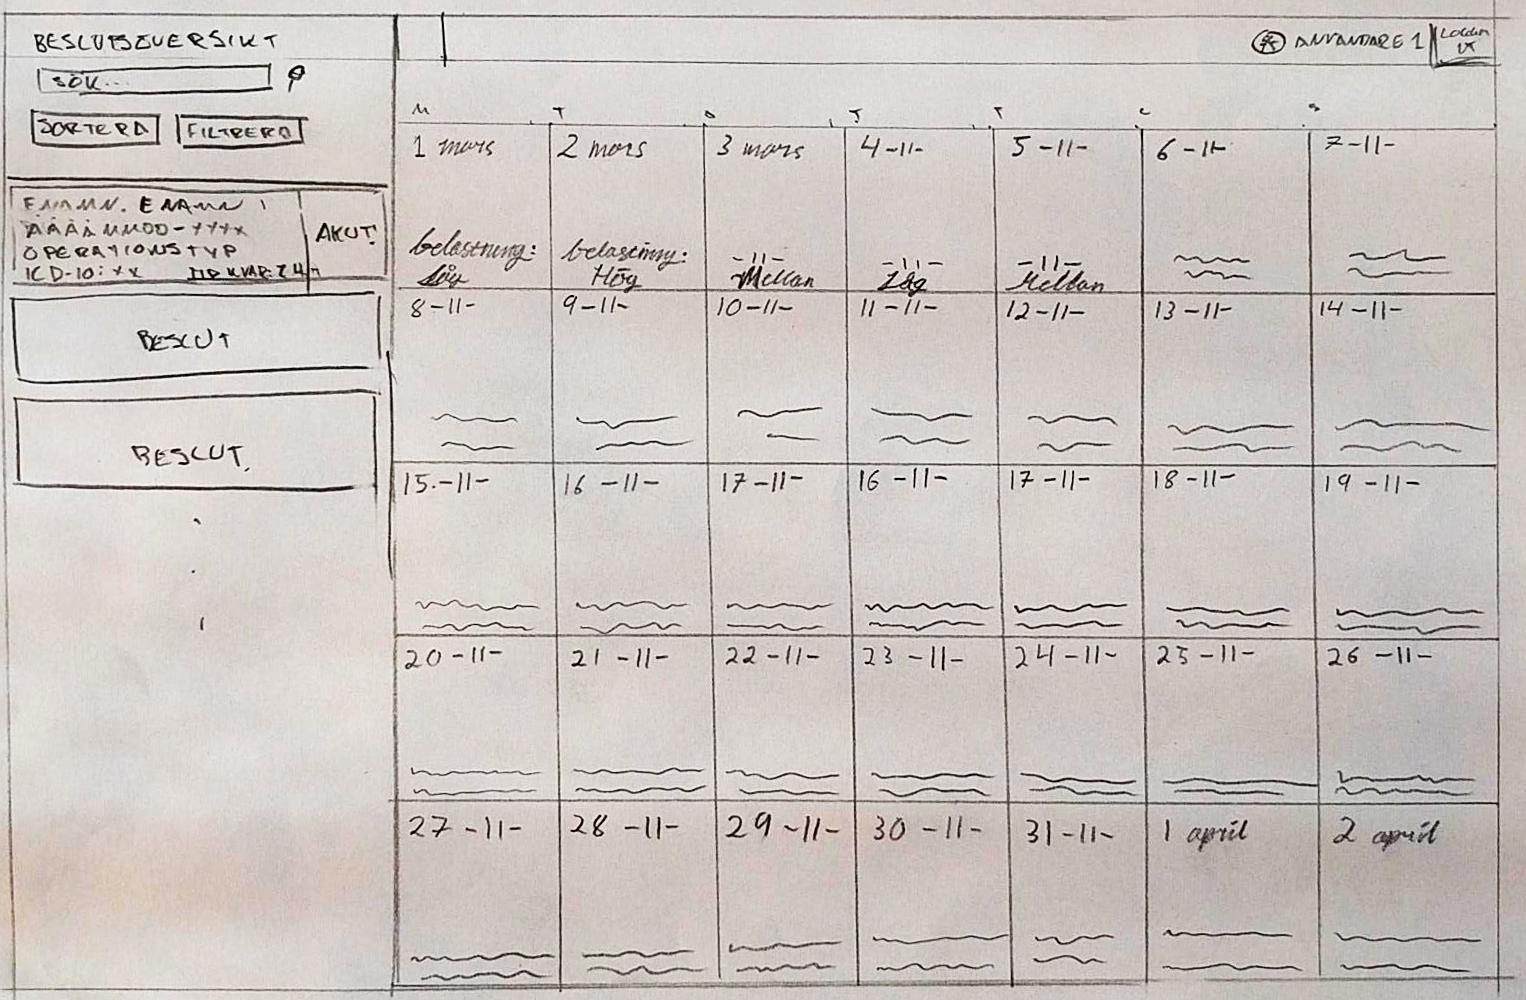
\includegraphics[width=\linewidth]{Figures/LoFi_no2.jpg}
  \caption{Sista LoFi-prototypen}
  \label{fig:LofiPic}
\end{figure}


Under projektets andra iteration utvecklades tre olika LoFi-prototyper. Dessa
LoFi-prototyper designades för att visa på olika designalternativ för
användargränssnittet. Ett exempel på detta är informationen som var med i listan
över beslutade operationer.

I en av prototyperna identifierades patienten som hörde ihop med beslutet med namn, den andra med personnummer. I den tredje LoFi-prototypen
fanns inget som identifierade patienten utan enbart information om vilken
typ av operation det var. På liknande sätt utvärderades olika sätt att
visualisera lediga tider i schemat samt olika sätt att anpassa sökparametrarna för en sökning efter lediga tider.

När prototyperna visades för kunden kunde alternativen sållas bort och en tydligare bild av behoven framträdde.
Till exempel gick det snabbt att konstatera att användarna ville ha både personnummer och namn för att identifiera patienter.

Den första iterationen av LoFi-prototyper användes sedan för att ta fram en ny
LoFi-prototyp med enbart mindre designalternativ som visades för tre olika
operationsplanerare. (Figur \ref{fig:LofiPic} illustrerar en bild av den sista Lofi-prototypen.)

\subsection{Grafiskt gränssnitt}
Då arbetet med prototyper var klart inleddes implementationen av designen i form av de grafiska komponenterna. Det här resulterade i en komplett webbsida med tre olika huvudkomponenter: sidopanelen, informationslisten och den huvudsakliga innehållsrutan.

Arbetsflödet i appen börjar med att användaren loggar in med sina inloggningsuppgifter. Därefter presenteras vyn som visas i figur \ref{fig:window}.

\begin{figure}
	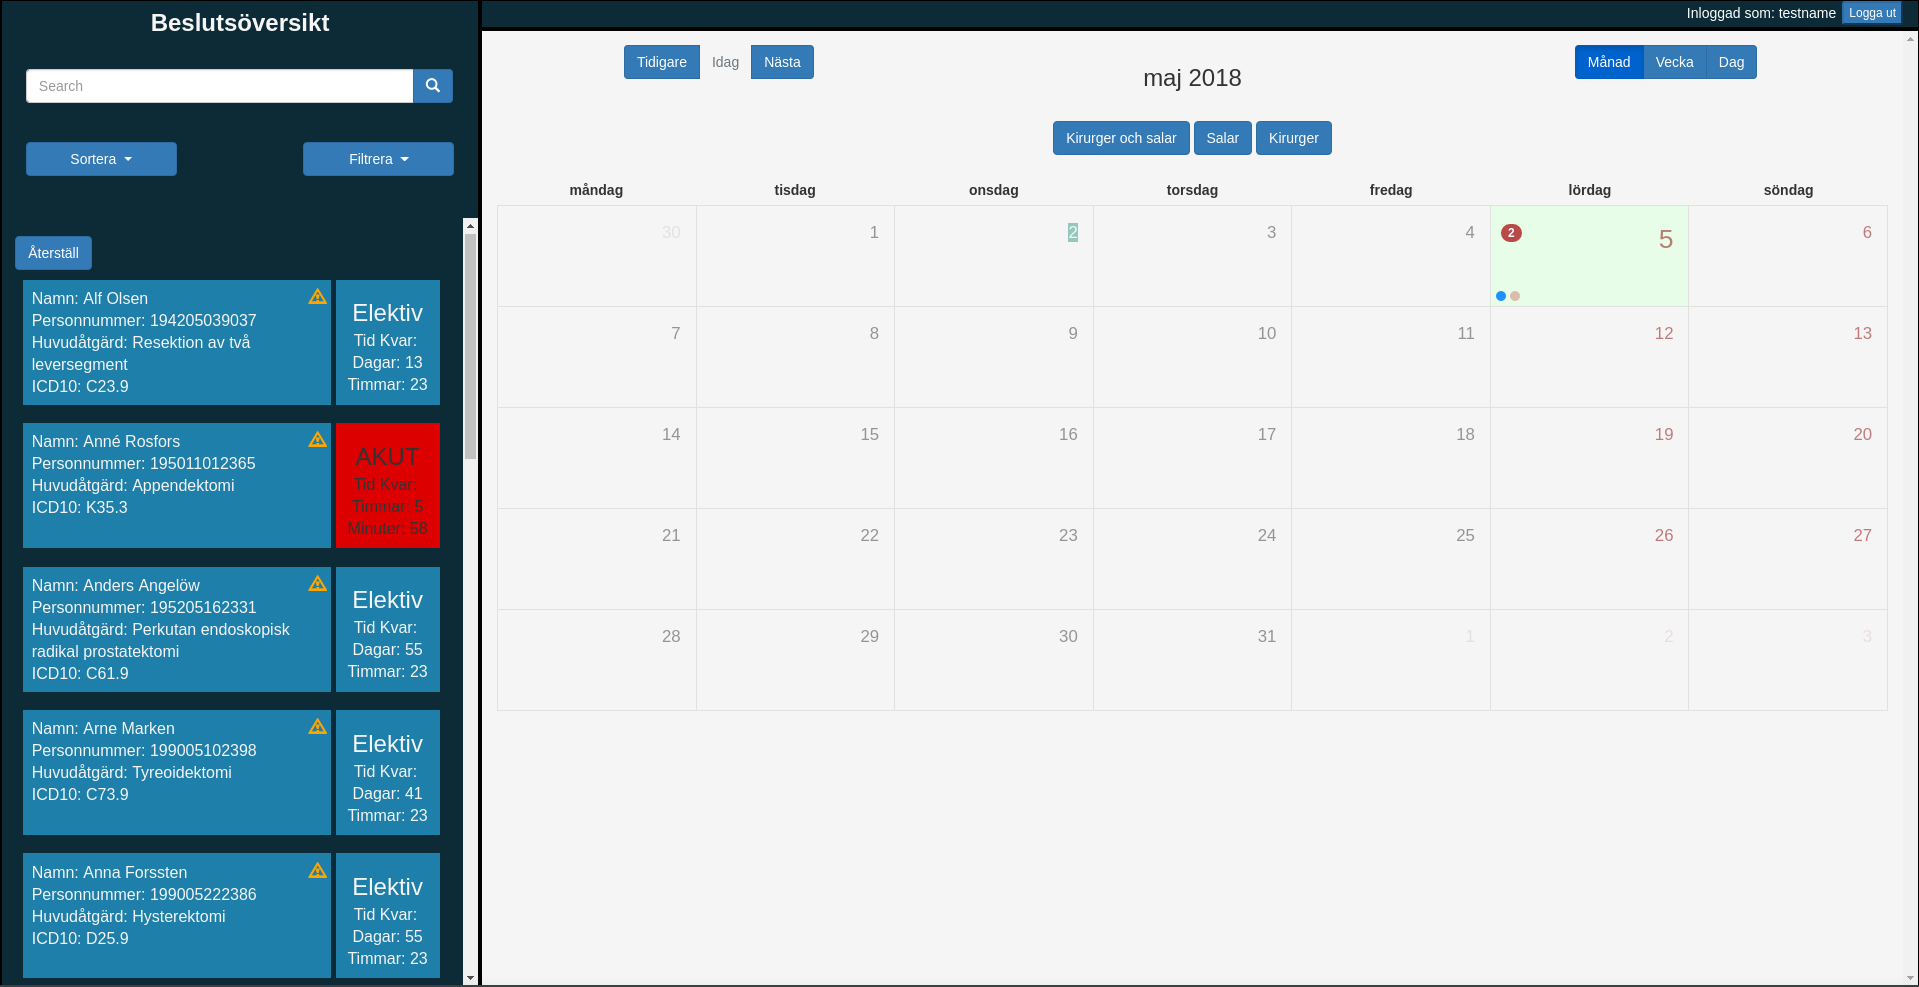
\includegraphics[width=\linewidth]{Figures/window.png}
	\caption{Gränssnittet}
	\label{fig:window}
\end{figure}


\subsubsection{Sidopanelen}
När användaren loggat in presenterar sidopanelen alla beslut som finns att planera (figur \ref{fig:beslutsvy}). Ett beslut visualiseras som ett kort som innehåller en mängd viktiga data som patientens namn och personnummer, hur långt det är innan operationen bör ske och även vilken typ av operation det gäller samt vad anledningen är till att operationen behövs. En akut operation är tydligt markerad med rött för att det enkelt ska gå att se att det är viktigt att boka in denna så snart som möjligt.

Det går även att söka i listan. Dessutom kan användare filtrera listan på olika kriterier och sortera den.

När användaren klickar på en patient så visas en detaljvy för patienten (figur \ref{fig:planeringsvy}). Här kan användaren se mer detaljerad information om beslutet som hur lång tid operationen beräknas ta, hur lång förberedelsetid som krävs med mera. Det går också att se en lista med alla de verktyg och material som krävs.

Längst ner finns det även en ruta med sökkriterier för att filtrera den schemavy som visas i huvudfönstret så att en ledig tid kan hittas.

\begin{figure}[H]
	\centering
	\begin{subfigure}[b]{0.4\linewidth}
		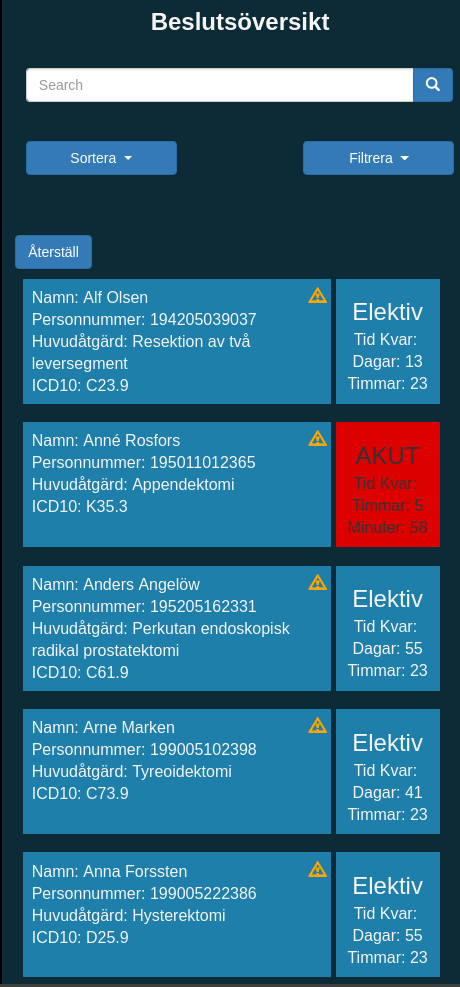
\includegraphics[width=\linewidth]{Figures/beslut.png}
		\caption{Beslutsvyn}
		\label{fig:beslutsvy}
	\end{subfigure}
	\begin{subfigure}[b]{0.4\linewidth}
		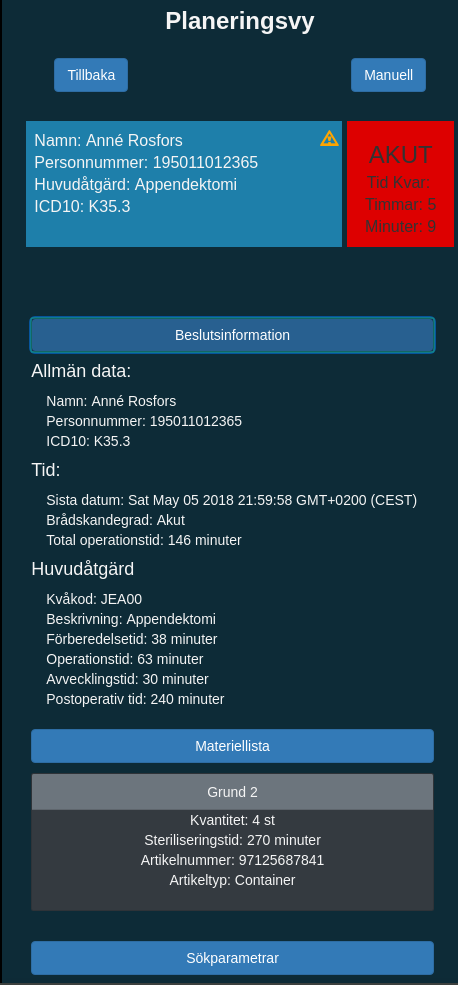
\includegraphics[width=\linewidth]{Figures/planning.png}
		\caption{Planneringsvyn}
		\label{fig:planeringsvy}
	\end{subfigure}
	\caption{Sidopanelens två vyer.}
	\label{fig:sidepanel}
\end{figure}


\subsubsection{Informationslisten}
Informationslisten är den smala rad längst upp gränssnittet i \ref{fig:window}.
Informationslisten är till för att alltid visa information om den patient som för tillfället håller på att bokas in. Så snart ett beslut har valts i sidopanelen så visas patientens namn och personnummer i informationslisten.

I informationslisten syns det också vilken användare som är inloggad längst till höger och där finns även en knapp för att logga ur aktuell användare.

\subsubsection{Huvudfönstret}
I huvudfönstret visas i grundutförandet en månadsvy över där det går att se hur många operationer som är inbokade på olika dagar. Om en dag markeras så visas fler detaljer över de operationer som är inbokade på den dagen. När en patient har valts i sidomenyn används månadsvyn för att välja vilken dag man vill boka in operationen. När en dag har valts skickas användaren vidare till spårvyn.

\subsubsection{Spårvyn}
Spårvyn, figur \ref{fig:track_view}, visar ett antal konfigurerbara spår där varje spår motsvarar schemat för en viss resurs på den valda dagen. Dessa spår visas brevid varandra för att enkelt visualisera de olika resurserna och på så sätt skapa en bra överblick över när de olika resurserna är lediga i relation till varandra. Det går att välja vilka resurser som ska visas, som salar, olika personer och verktyg.

\begin{figure}[H]
	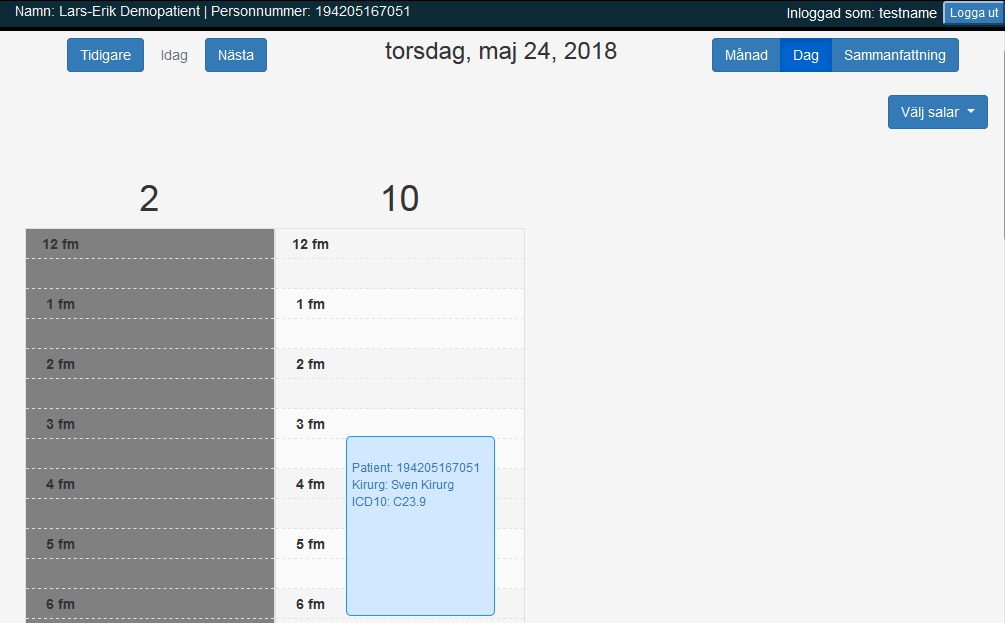
\includegraphics[width=\linewidth]{Figures/track_view.png}
	\caption{Spårvyn}
	\label{fig:track_view}
\end{figure}

\subsection{Systemanatomi}
I första iterationen togs det fram en systemanatomi (se figur \ref{fig:Systemanatomi}) som användes under projektets gång som ett hjälpmedel för att strukturera upp arbetet under utvecklingen. Den gav en översiktlig bild av vilken funktionalitet produkten skulle innehålla och hur de olika delarna samverkade med varandra. Utöver detta presenterades den i ett tidigt skede för kunden i syfte att säkerställa att projektgruppens syn på systemet stämde överens med kundens.

\begin{figure}[H]
    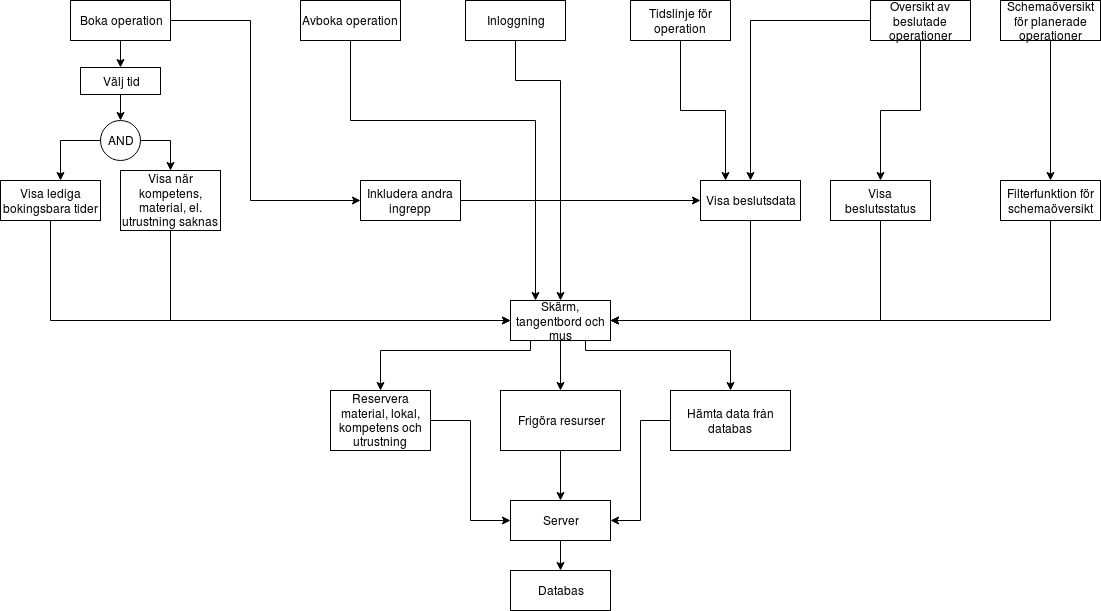
\includegraphics[width=\textwidth,height=.4\textheight]{Figures/Systemanatomi.png}\\
    \caption{Systemanatomi}
    \label{fig:Systemanatomi}
\end{figure}

\subsection{Värde för kund}
Den produkt som har skapats är ett lättöverskådligt schemaläggningssystem för operationer. Systemet matchar väl den initila målbilden. Sedan har nya upptäckter under projektets gång gjort att systemet förmodligen behöver kompleteras avsevärt för att vara praktiskt användbart. Detta är dock inte ett stort problem då syftet var att skapa en prototyp (se \ref{sec:syfte}).

Dokumentationen och processen under projektet har varit minst lika viktig för att ta reda på vad som kommer och inte kommer att fungera och ger stor insikt i hur systemet kan se ut och hur produkten kan förbättras i framtiden.

Vår förhoppning är att de arbetsdokument som vi tagit fram i gruppen som stöd under arbetet kan vara till hjälp för den fortsatta utvecklingen. Detta tillsammans med de officiella dokumenten borde skapa en solid teoretisk kunskapsgrund för vidareutveckling.

Vad gäller faktisk programvara så tror vi starkt på att det finns funktioner och element i vår design som bidrar till en ny syn på schemaläggning och som kan komma till användning antingen som vi implementerat dem eller som inspiration för andra nya sätt att bygga upp systemet.

Totalt sett medför detta att Region Östergötland kommer att ha en bra grund att utgå ifrån då deras projekt startar. Både projektledaren och andra aktörer för det större projektet kommer att kunna ta med sig många erfarenheter från det här projekt i och med att flera av dem har varit så delaktiga i vår process genom flera möten.

\section{Gemensamma erfarenheter}
I denna del kommer gruppens gemensama erfarenheter presenteras.

\subsection{Tekniska erfarenheter}
Under projektet har medlemmarna fått stor erfarenhet av webbprogrammering då ingen hade någon större erfarenhet av detta sedan tidigare. Gruppen har fått sätta sig in i HTTP-protokoll, databaser och ett flertal programspråk och ramverk. Även versionshantering med Git och GitLab har gruppen fått fördjupad kunskap inom.

Vid utveckling av front-end lärde sig gruppen att använda ramverket Angular och att programmera i HTML, CSS och TypeScript. För back-end behövde medlemmarna istället sätta sig in i JavaScript, MySQL-databaser och miljön Node.js med ett flertal tillhörande bibliotek.

Förutom tekniska erfarenheter har gruppen fått en större förståelse för hur sjukvården fungerar och att ett bra IT-system kan göra stor verklig skillnad. Gruppen har även fått praktiskt erfarenhet av att utöva Scrum. Det har varit seminarier där presentation och opponering ingick.

\subsection{Kommunikation och planering}
Det som förmodligen fungerat sämst i gruppen är kommunikation och planering. Det innebär inte på något vis att detta har gått dåligt. Däremot är det i detta avseende som gruppen har fått jobba hårdast för att lyckas. Arbetetes effektivitet är kraftigt beroende av dessa två komponenter. Det som gruppen har insett är att om det inte finns en bra plannering så vet inte deltagarna vad de ska göra. Men ett annat problem är att det måste kommuniceras tydligt hur långt i planneringen de olika medlemmarna kommit. För att lyckas med detta så har gruppen jobbat hårt med både kommunikation och plannering och varje gång någon av delarna har fallerat så har det disskuterats och förbättrats.
\subsection{Dokumentation}
Dokumentation tar otroligt mycket tid att producera. Detta var något som gruppen inte var berädda på och till följd av detta så gjordes vissa övergripande planneringsmisstag. Det hade tillexempel varit bra att börja med programmeringen tidigare, det vill säga innan dokumenten var färdigskrivna.
Däremot så har gruppen ochså insett den verkliga potentialen med bra dokument som beskriver projekter. Då gruppen väl började med programmeringen så gick det väldigt snabbt och effektivt eftersom så mycket av strukturen redan var bestämd.
\subsection{Samlad kompetens}
En annan stor  erfarenhet som kom utav detta projektet var en insikt i hur mycket som kan åstakommas genom att samla ihop de olika medlemmarnas olika kompetenser. Inte bara tidigare kunskap utan även genom aktivt delande av ny kunskap. Alla medlemmarna i detta projektet har uttrykt en känsla av ökat självförtoende i sin kapacitet som ingengör under detta projekt.

\subsection{Nyttan för kommande projekt}
Av det som pressenterats i detta stycket så är det främst de tre sista rubrikerna som gruppen bedömmer som viktiga att ta med sig in i kommande projekt. Det är viktigt att hålla en bra stuktur för regelbunden planering och en bra stuktur för koninuerlig kommunikation. Dokumentation tar tid men är värt det i längden. Däremot är det viktigt att inte fastna utan att komma vidare i tid.
Till sist så tar gruppen också med sig att samlad kompetens är en otrolig tillgång och om den används och delas rätt så skapar det självsäkra individer som tillsammans bildar en stabil grupp.



\section{Översikt över individuella bidrag}
I denna del presenteras deltagarnas individuella bidrag översiktligt.

\subsection{Teamledarens roll kombinerad med Scrum-metodik av Adam Andersson}
I Scrum-metodik finns det ingen ledare utan alla medlemmar i teamet är med och tar de beslut som ska göras. Denna studie är till för att utvärdera om det går att kombinera rollen teamledare med en projektgrupp som använder sig av Scrum-metodik och ändå kunna behålla syftet med de båda.
\subsection{Versionshantering för ett mindre mjukvaruutvecklingsprojekt av Björn Hvass}
Rapporten undersöker hur versionshantering kan användas i ett mindre mjukvaruutvecklingsprojekt samt redogör för om det går att använda en arbetsmetodik effektivt i den här typen av projekt.

\subsection{Effektivt val av aktörer för kravinsamling av Christoffer Sjöbergsson}
Kan en strukturerad metod för urval och prioritering av krav och aktörer förbättra kraven i ett mindre mjukvaruprojekt?
\subsection{Jämförelse mellan TypeScript och JavaScript av Henrik Lindström}
Denna rapport jämför språken TypeScript och JavaScript baserat på erfarenheter från projektet och litteratur. Undersökningen fokuserar på TypeScript och JavaScripts olika typsystem - statisk respektive dynamisk typning. Inom detta är det påverkan på feldetektering, kodförståelse och produktivitet hos de två språken som behandlas.
\subsection{Angular som webbutvecklingsplattform av Martin Persson}
Denna rapport utvärderar vad valet av Angular som webbutvecklingsplattform tillfört projektet och vilka faktorer man bör ta hänsyn till vid val av ramverk till webbutvecklingsprojekt som liknar detta.  
\subsection{Prototyputveckling i ett kandidatprojekt av Niclas Byrsten}
Denna rapport undersöker hur prototyper användes i projektet och vilka slutsatser som kan dras baserat på gruppens erfarenheter.
\subsection{Kvalitetsförsäkrande metoder i ett småskaligt mjukvaruprojekt av Tor Utterborn}
En undersökning om kvalitetsförsäkrande metoder i ett småskaligt mjukvaruprojekt där de två metoderna som undersökts är användandet av ramverket Angular samt de statiska kod-analysverktyget TSLint.
